% plan-failure-bench paper, formatted for TMLR.
% Compile with latexmk -pdf (see paper/Makefile).
% The results tables are generated by tools/build_paper_results.py and
% must never be edited by hand. See paper/STATUS.md for the current
% state of each section.

\documentclass[10pt]{article}

% TMLR style (official kit from github.com/JmlrOrg/tmlr-style-file,
% vendored as tmlr.sty, tmlr.bst and fancyhdr.sty). Committed builds use
% the preprint option: named author and no TMLR header, the version for
% arXiv and Zenodo. For the TMLR submission, remove the option: the
% author block becomes "Anonymous authors", the header reads "Under
% review as submission to TMLR", and the abstract's closing line cites
% the anonymised mirror instead of the repository.
\usepackage{tmlr}
\usepackage[utf8]{inputenc}
\usepackage{microtype}
\usepackage{booktabs}
\usepackage{graphicx}
\usepackage[hidelinks]{hyperref}
\usepackage{url}

\graphicspath{{../docs/img/}}

\newcommand{\benchname}{plan-failure-bench}

% Anonymised mirror of the repository for double-blind review, served
% from the anon-mirror branch (no compiled preprint, identifiers
% scrubbed by the mirror service). Used only by the anonymous build.
\newcommand{\anonrepourl}{https://anonymous.4open.science/r/plan-failure-bench-2217}

\title{\benchname: A Machine-Checkable Benchmark\\of How Language Model Planners Fail}
\author{\name Anonymous authors}

% Used by the TMLR header only once accepted; placeholders until then.
\def\month{MM}
\def\year{YYYY}
\def\openreview{\url{https://openreview.net/forum?id=XXXX}}

\begin{document}
\maketitle

\begin{abstract}
Planner evaluations for language models usually report a success
rate, rely on labels written by hand, and often score with a human or
LLM judge. We propose construction rules that remove all three and
demonstrate them in \benchname{}. Each of 60 instructions over two
symbolic indoor environments either admits a valid plan or plants one
trap from six families (unreachable goal, missing capability, ambiguous
referent, precondition, sequencing, constraint), and each label carries
a proof that continuous integration re-checks on every commit. Models
answer in a small JSON action language with explicit infeasible and
clarify responses, so a deterministic checker scores every answer and
every detection count is reported with its false positive count on
feasible instructions. The checker is differentially tested against an
independent PDDL toolchain, and every instruction also appears in a
semantically obfuscated form produced by a versioned, invertible
renaming. At this scale the results on four models are hypotheses. The
models fail in different ways; the obfuscation versioning exposed one of
our own apparent findings as a token artefact; no model distinguishes a
missing capability from an unreachable goal; and the strongest model
tested, Gemini 3.6 Flash, nearly clears the suite in both conditions,
so the failure findings apply to smaller models.
\makeatletter\if@preprint
This is a working paper; every number in it is reconstructible from
the repository.
\else
Every number in this paper is reconstructible from the anonymised
repository, provided as supplementary material and mirrored at
\url{\anonrepourl}.
\fi\makeatother
\end{abstract}

\section{Introduction}

When a household robot is driven by a language model planner, the
most dangerous failures are confident ones: the model that plans a
route through a room it was told never to enter, or
fetches one of two identical cups without asking which. Before asking
whether a language model plans well, a benchmark should ask whether the
model notices when planning is the wrong response altogether.

\benchname{} makes that question checkable by machine. The
contribution is a way of constructing planner evaluations: every
scoring decision is mechanical, every ground-truth label carries a
proof, and every number in this paper is generated from committed run
records. The grid of four models and two environments reported here
demonstrates the method at small scale (30 instructions per
environment, models chosen by free-tier access), so its findings are
stated as hypotheses. The construction rules ensure that those
hypotheses cannot come from a judge, a mislabelled instruction, or a
transcription error, and Section~\ref{sec:results} describes two
artefacts the method caught in its own first obfuscation scheme. The
rules:

\begin{enumerate}
\item \textbf{Finite symbolic worlds.} States are sets of ground atoms
  with no numerics, so every label can be proved mechanically.
\item \textbf{Proof obligations in continuous integration.} Every seed's
  label carries a mechanical proof (a validating reference plan, an
  unreachability proof from a sound abstraction, a capability grant that
  flips infeasibility, or exhaustive referent bindings), re-proved on
  every commit by 589 tests.
\item \textbf{Refusal and clarification as first-class answers.} The
  response language contains \texttt{infeasible(reason)} and
  \texttt{clarify(candidates)} terminals, so detection is scored
  mechanically and always reported alongside the paired false positive
  count on feasible instructions.
\item \textbf{A semantically obfuscated condition.} Content words are
  renamed by a versioned bijection applied to the prompt and inverted on
  the response, separating state tracking from lexical pattern matching
  while the checker scores only the canonical world.
\item \textbf{Two structurally contrasting environments.} The second
  environment varies topology and constraint structure specifically to
  test whether findings from the first are artefacts of one map.
\item \textbf{Open, replayable records, and no transcribed numbers.}
  Every run is committed as one JSON record per seed, both scoring
  policies re-score offline without model calls, model names resolve
  through a committed manifest of exact API checkpoints, and the
  results tables in this paper are generated from the records.
\end{enumerate}

\section{Related work}

\textbf{Evaluating LLM planning.} PlanBench established systematic
evaluation of LLM planning over symbolic domains and its successors
have repeatedly found generation weak \citep{valmeekam2023planbench,
valmeekam2023planning}. The same line introduced Mystery Blocksworld,
obfuscating a familiar domain to separate reasoning from lexical
recall, and found that plan generation collapses; \benchname{} inherits
that manipulation, applies it as a versioned bijection, and asks which
\emph{judgements} survive semantic removal as well as whether
generation does. Unsolvability recognition
itself is not new: PlanBench ships unsolvable instances scored by true
and false negative rates, and \citet{valmeekam2024strawberry} report
o1-preview explicitly recognising 27\% of unsolvable Blocksworld
instances, 16\% under randomised obfuscation, while wrongly declaring
11.5\% of solvable obfuscated instances impossible. What \benchname{}
adds is breadth and pairing: six trap families under one response protocol, detection always paired with
false positives, and per-seed proof obligations. Pipeline alternatives such
as LLM+P hand the search problem to a classical planner and use the
model only for formalisation \citep{liu2023llmp}; \benchname{} instead
measures the model as the planner, because the failure modes of that
configuration are what the benchmark exists to characterise.

\textbf{Feasibility, ambiguity, and safety as separate literatures.}
Each trap family here has a single-family predecessor. Plancraft
includes intentionally unsolvable crafting tasks scored mechanically:
given an explicit impossible action, its best model reaches F1 0.71 at
declaring impossibility, and models become overeager, trading success
on solvable tasks for refusals \citep{dagan2025plancraft}. AmbiK pairs
every ambiguous kitchen instruction with an unambiguous counterpart
and scores whether detection methods can tell the two apart
\citep{ivanova2025ambik}, and the asking-for-help line, KnowNo's
calibrated uncertainty and CLARA's command classification, trades help
requests against success guarantees \citep{ren2023knowno,
park2024clara}. Two 2026 benchmarks make the pairing suite-wide in
the tool-use setting: TREK pairs 533 feasible travel-planning tasks
with 267 provably infeasible ones whose causes are typed (route,
entity, budget), scores with deterministic rules and no LLM judge,
and grades a bare refusal strictly below one that names the right
cause \citep{qi2026trek}; AgentAbstain pairs every should-abstain
task with a should-act variant differing in exactly one perturbation
across eight scenarios, so that no constant policy can exceed 50\%
paired accuracy, though an LLM judge scores the terminal response
\citep{liu2026agentabstain}. Paired or trade-off measurement
therefore exists within single families and, in tool-use domains,
suite-wide, including the false impossibility claims measured by
\citet{valmeekam2024strawberry}; \benchname{} carries the pairing
into embodied planning across six trap families under one protocol. SafeAgentBench shows embodied agents complying with
hazardous instructions and documents the over-refusal trade-off
directly, a safety module raising rejection of safe tasks alongside
hazardous ones \citep{yin2024safeagentbench}; HomeBench evaluates
valid and invalid instructions in smart home device control, where
even frontier models fail badly on invalid multi-device cases
\citep{li2025homebench}. XSTest documents the chat-model analogue of
over-refusal, driven by surface features of safe prompts
\citep{rottger2024xstest}, and Semantic Denial of Service attacks show
robot refusal triggering on injected surface-level safety phrases
regardless of physical state \citep{steinberg2026semanticdos},
adversarial evidence of the same anchoring our obfuscation
manipulation measures. The nearest neighbour to our aims is the
Yes-Man Syndrome benchmark \citep{yeke2026yesman}, which measures
abstention by embodied agents over ambiguous, physically infeasible,
false-premise, and sensing-unresolvable instructions. Its instructions
are generated by deterministic constraint derivation, but its scoring
uses an LLM judge, it measures only whether agents abstain when they
should, with no false positive column for valid instructions, and it
has no semantic obfuscation condition; its categories all target
abstention, while half of \benchname{}'s taxonomy consists of feasible
instructions carrying planted execution traps, which is what makes the
planted versus observed confusion matrix possible. To our knowledge no
prior benchmark manipulates surface semantics while measuring refusal,
the manipulation behind our finding that refusal behaviour is anchored
to surface semantics in opposite directions for different models.

\textbf{Error taxonomies and ground truth.} The Embodied Agent
Interface catalogues fine-grained error types across goal
interpretation, decomposition, sequencing, and transition modelling
\citep{li2024embodied}. \benchname{} differs in direction: instead of
classifying observed errors after the fact, it plants exactly one
labelled trap per instruction and reports the confusion matrix between
planted and observed, asking whether models fail as predicted. That
requires ground truth that can be checked independently, which places
this work in the plan-validation tradition of VAL \citep{howey2004val}:
verdicts come from a deterministic checker differentially tested
against an independent PDDL executor, pyperplan
\citep{alkhazraji2020pyperplan}, labels are proofs re-run in continuous
integration, and no human or model judgement appears anywhere in the
scoring loop. Plancraft also scores mechanically inside its crafting
environment, TREK's evaluator is deterministic rules over its travel
knowledge base, and SIMMER validates cooking plans with a
state-machine executor over a curated symbolic kitchen world; its
latent failures, flawed plans that execute without immediate
feedback, are single-domain kin to our silent-violation constraint
seeds, though all of its tasks are solvable, so refusal, paired false
positives, and semantic manipulation are out of its scope
\citep{lu2026simmer}. RoboBench, by contrast, delegates plan
feasibility scoring to a multimodal model acting as a world simulator
\citep{luo2025robobench} and the Yes-Man benchmark scores with an
LLM judge. What no benchmark
above combines is judge-free scoring with per-seed proof obligations
re-run in continuous integration and differential testing of the
checker itself.

\textbf{Proving that no plan exists.} Our infeasibility labels rest on
a standard result in classical planning: if a projection of a task onto
a subset of its variables has no solution, neither does the task.
\citet{backstrom2013unsolvable} search such projections to detect
unsolvable instances, and \citet{hoffmann2014distance} design
merge-and-shrink abstractions for the same purpose. Our abstraction is
simpler: for each goal literal it tracks the robot, the doors, and one
item exactly and over-approximates every other item, which is enough
to prove every infeasible label in both suites.
\citet{eriksson2017certificates} note that plans are routinely checked
by independent validators while claims of unsolvability were not, and
propose certificates that a separate verifier can check. Our
unreachability proofs are checked only by our own code; emitting such
certificates would give them the independent check our plans receive.

\textbf{Measurement validity and judge reliability.} The construction
rules in the introduction respond to documented pathologies of
current evaluation practice. A systematic
review of 445 LLM benchmarks found nearly every one weak on at least
one construct validity criterion, the operationalisation of abstract
phenomena often insufficient, and issued eight recommendations
including defining the phenomenon, preparing for contamination, and
justifying construct validity \citep{bean2025validity}; \benchname{}
answers the narrower internal-validity question by proof, since what
each instruction measures is its planted, machine-proved label. On judges, a systematic evaluation of 21 LLM
judges over roughly 541{,}000 judgments finds that raw exact-match
agreement overstates discriminative ability (Cohen's kappa 33.8 to
41.3 percentage points lower on MT-Bench), that judge rankings shift
by up to 14 positions across benchmarks, and that production-deployed
judges combine near-perfect test-retest reliability with severe
position bias \citep{norman2026judges}; \benchname{} scores with no
judge anywhere, so those pathologies do not apply. Shallow-cue
exploitation has also been measured directly: simple classifiers over
answer n-grams score highly on several multiple-choice benchmarks
while lacking the capability being tested
\citep{pacchiardi2024cleverhans}. The obfuscated condition answers the
same concern by construction, removing the surface cues while provably
preserving task structure.

\section{Benchmark design}

\subsection{World model}

An environment is a set of rooms connected by doors (open, closed, or
locked), items with categories and properties located in rooms, a robot
with a capability profile over a fixed action vocabulary (goto, open,
close, pick, place, and optionally unlock), a single-slot gripper, and
trajectory invariants that must hold in every state along a plan. Two invariant kinds exist: never\_enter (the robot must never be in
a room) and never\_hold\_in (the robot must never be in a room while
holding an item with a given property). Invariant text is shown to the
model verbatim, so the model is told every constraint it is scored
against. State is a finite set of ground atoms over a fixed object
universe with no numerics, so the state space is finite.

\subsection{Task language}

Models receive a fixed rendering of the environment and one natural
language instruction, and must answer with exactly one JSON object: a
\texttt{plan} (a list of actions), \texttt{infeasible} with a reason
from \{unreachable, missing\_capability, constraint\}, or
\texttt{clarify} with candidate referents. The strict scoring policy,
the headline, requires exactly a response-shaped JSON object; a
documented lenient policy re-scores stored records offline by extracting
the first response-shaped JSON object, separating format discipline from
planning ability.

\subsection{Trap taxonomy and proof obligations}

We call each labelled instruction a \emph{seed}, and the 30 seeds of
one environment a \emph{suite}. Each seed either admits a valid plan or
plants exactly one trap.
Labels carry these proof obligations, re-proved on every test run:

\begin{itemize}
\item \textbf{valid}: a reference plan validates under the checker and
  under independent PDDL execution, and no infeasibility proof exists.
\item \textbf{unreachable\_goal}: provably unreachable under a sound
  over-approximating abstraction, and still unreachable with the full
  action vocabulary granted.
\item \textbf{missing\_capability}: provably unreachable under the
  robot's profile, not provable once a named capability is granted, and
  a capability reference plan validates in the augmented environment.
\item \textbf{ambiguous\_referent}: at least two same-category bindings,
  each with a validating reference plan and no infeasibility proof; the
  expected answer is clarify with exactly the category's members.
\item \textbf{precondition\_trap} and \textbf{sequencing\_trap}: the
  goal is feasible (reference plan validates); a decoy plan documenting
  the intended error produces exactly the declared trap verdict.
\item \textbf{constraint\_trap}: either feasible with a decoy that
  executes fully, achieves the goal, and silently breaches an invariant,
  or provably infeasible solely because of an invariant.
\end{itemize}

A \emph{decoy plan} is the tempting wrong plan a trap is built around.
Precondition and sequencing traps together are the \emph{ordering
traps}, seven per suite. Four seeds recur by name in the results. The
\emph{silent-violation} seed is the feasible constraint seed, whose
decoy executes fully and reaches the goal while breaching an invariant;
the \emph{compound} constraint seed asks for two items, only one of
which may be carried to the target; two missing-capability seeds are
\emph{locked-door} seeds, sealed behind a door this robot cannot
unlock; and the third is the \emph{inexpressible-verb} seed, which asks
for an action no robot has, such as mopping.

A trap verdict on a feasible seed shows that the model missed the trap.
It does not show that the model took the decoy: precondition\_violation
is the verdict for any plan that fails early, whatever the cause, so an
observed precondition\_violation on a precondition trap is consistent
with the decoy but does not identify it.

\subsection{Environments}

\textbf{house\_01}: seven rooms, six doors, ten items, two
never\_hold\_in invariants (each property carried by exactly one item),
a doorless cellar whose isolation the environment description states
outright, and a locked store room behind the withheld unlock capability.
It contains one cycle (kitchen, hallway, living room), passable only
through a closed door.

\textbf{office\_01}: nine rooms, eight doors, eleven items, built to
contrast with house\_01 in structure. A
five-room ring reachable through open doors makes route choice pervasive.
A never\_enter room sits on the ring, so the short route between
reachable rooms can silently violate an invariant by movement alone. A
never\_hold\_in property is carried by three items rather than one. A
two-room annex is disconnected from the rest of the map, but both its
rooms have doors, so no ``has no doors'' statement appears and the
isolation must be inferred from the connection list. Ambiguous referent
candidates can sit in different rooms, and one decoy traps the
single-slot gripper itself. Both suites plant the same label
distribution (9 valid, 4 unreachable, 3 missing capability, 3 ambiguous,
4 precondition, 3 sequencing, 4 constraint), keeping confusion matrix
columns comparable across environments.

\subsection{Obfuscated condition}

Semantic content words (rooms, doors, items, categories, properties,
actions, door states) are replaced by deterministic nonsense tokens;
structural vocabulary (room, door, item, gripper) and the response
protocol are retained. The renaming is a bijection applied to the
assembled prompt and inverted on the model's raw response before
checking, so the checker, the seeds, and every label proof operate only
on the canonical world and no second world model exists to drift.
Version 1 tokens were confusable enough that model copy errors were
indistinguishable from hallucination; version 2 tokens guarantee unique
opening syllables and pairwise edit distance of at least three. Every
record stores the obfuscation version it was produced under.

\section{Ground truth guarantees}

The checker simulates each plan step by step and assigns exactly one
verdict: valid, precondition\_violation, constraint\_violation,
goal\_not\_achieved, hallucinated\_entity, unavailable\_action, or
malformed, plus the two terminals. It is differentially tested against
pyperplan over hand-written trap plans and hundreds of seeded random and
guided plans, with first-failing-step agreement required. A second
compilation turns both invariant kinds into STRIPS preconditions, the
standard compilation of PDDL~3 \emph{always} constraints over state
atoms, and there the first inapplicable step must equal the checker's
first breach step, so the oracle covers constraint verdicts as well as
executability and goal satisfaction. Infeasibility labels are proofs from a per-literal
over-approximating abstraction whose direction is sound: every real
trajectory has an abstract counterpart, so goals the abstraction cannot
reach are truly unreachable, and reachable-looking goals are proved
feasible constructively by reference plans, never by the abstraction.

\section{Experimental setup}

Four models, all under a fixed prompt at temperature 0 with one decode
per seed, each covering both suites in both conditions: Llama 3.3 70B
(Groq API), Qwen 2.5 7B Instruct (run locally through Ollama as the
4-bit Q4\_K\_M quantization of the \texttt{qwen2.5:7b-instruct} tag),
Gemini 3.1 Flash Lite, and Gemini 3.6 Flash (both Gemini API; the
latter a reasoning model). Each request carried the prompt
as one user message, temperature 0, and the output limit in
Table~\ref{tab:models}, and nothing else. No JSON mode or structured
output constraint was used, so format failures measure the models'
unconstrained output. No reasoning or thinking parameter was sent, so
both Gemini models ran with the provider's default thinking, and their
reasoning tokens are not recorded. Temperature 0 does not make a hosted
API replay identically, so each single decode is one sample of the
model's behaviour. Seven of the 1350 committed responses stop at the
output limit mid-answer, all malformed under the strict policy
(\texttt{tools/audit\_truncation.py} lists them). One is in a
superseded version 1 run. Of the six in the current grid, five are
Llama office\_01 responses from which lenient extraction recovers an
earlier plan, and one is a Flash Lite plan that moves between two
rooms 483 times before the limit cuts it off.
Table~\ref{tab:models} records the exact API checkpoint behind each
run alias; every committed record carries the alias, and records
written from now on carry the checkpoint string itself, so the mapping
from a table row to the model that produced it is recorded in the
repository. The superseded version 1 obfuscated runs of Llama and
Qwen are retained and marked in the tables, because the artefacts they
exposed are part of the methodology's history.

\begin{table}[t]
\centering
\small
% Generated by tools/build_paper_results.py from
% configs/model_manifest.json. Do not edit by hand.
\begin{tabular}{lllr}
\toprule
Model & Run alias in records & API checkpoint & Output limit \\
\midrule
Llama 3.3 70B & \texttt{groq\_llama70b} & \texttt{llama-3.3-70b-versatile} & 2000 \\
Qwen 2.5 7B (Q4\_K\_M) & \texttt{local\_qwen} & \texttt{qwen2.5:7b-instruct} & 2000 \\
Gemini 3.1 Flash Lite & \texttt{gemini\_flash\_lite} & \texttt{models/gemini-3.1-flash-lite} & 8000 \\
Gemini 3.6 Flash & \texttt{gemini\_flash} & \texttt{models/gemini-3.6-flash} & 8000 \\
\bottomrule
\end{tabular}

\caption{Model aliases in the committed records, the exact API
checkpoints they called, and the output token limit of every request,
generated from the committed manifest.}
\label{tab:models}
\end{table}

\section{Results}
\label{sec:results}

Numbers below are counts under the lenient extraction policy, one
decode per seed at temperature 0 unless a paragraph says otherwise,
with strict format failures reported per run. At $n=30$ per condition
they are hypotheses. Table~\ref{tab:runs} is
generated directly from the committed records.

\begin{table}[t]
\centering
\footnotesize
\setlength{\tabcolsep}{3.5pt}
% Generated by tools/build_paper_results.py from results/*.jsonl.
% Do not edit by hand; rerun the tool after any completed run.
\begin{tabular}{llllrrrrr}
\toprule
Model & Environment & Condition & Note & \shortstack[l]{Format\\failures} & \shortstack[l]{Traps\\detected} & \shortstack[l]{Exact\\reasons} & \shortstack[l]{False\\positives} & \shortstack[l]{Valid\\solved} \\
\midrule
Llama 3.3 70B & house\_01 & plain &  & 18/30 & 9/13 & 6 & 3/17 & 5/9 \\
Llama 3.3 70B & house\_01 & obfuscated (v1) &  & 23/30 & 11/13 & 9 & 1/17 & 1/9 \\
Qwen 2.5 7B & house\_01 & plain &  & 3/30 & 2/13 & 0 & 0/17 & 2/9 \\
Qwen 2.5 7B & house\_01 & obfuscated (v1) & superseded & 5/30 & 3/13 & 1 & 0/17 & 1/9 \\
Qwen 2.5 7B & house\_01 & obfuscated (v2) &  & 10/30 & 3/13 & 1 & 3/17 & 1/9 \\
Gemini 3.1 Flash Lite & house\_01 & plain &  & 0/30 & 12/13 & 8 & 4/17 & 6/9 \\
Gemini 3.1 Flash Lite & house\_01 & obfuscated (v2) &  & 0/30 & 7/13 & 6 & 1/17 & 5/9 \\
Qwen 2.5 7B & office\_01 & plain &  & 4/30 & 1/13 & 0 & 0/17 & 2/9 \\
Qwen 2.5 7B & office\_01 & obfuscated (v2) &  & 13/30 & 3/13 & 2 & 2/17 & 3/9 \\
Gemini 3.1 Flash Lite & office\_01 & plain &  & 1/30 & 10/13 & 6 & 7/17 & 4/9 \\
Gemini 3.1 Flash Lite & office\_01 & obfuscated (v2) &  & 1/30 & 5/13 & 4 & 2/17 & 2/9 \\
\bottomrule
\end{tabular}

\caption{Every complete committed run. Format failures are strict-policy
malformed responses out of 30; all other columns use lenient extraction.
Traps detected counts the 13 seeds per suite whose expected answer is a
terminal, and should be read with the paired false positives on the 17
feasible instructions. Exact reasons counts detections whose reason code
or candidate set was exactly right.}
\label{tab:runs}
\end{table}

\begin{figure}[t]
\centering
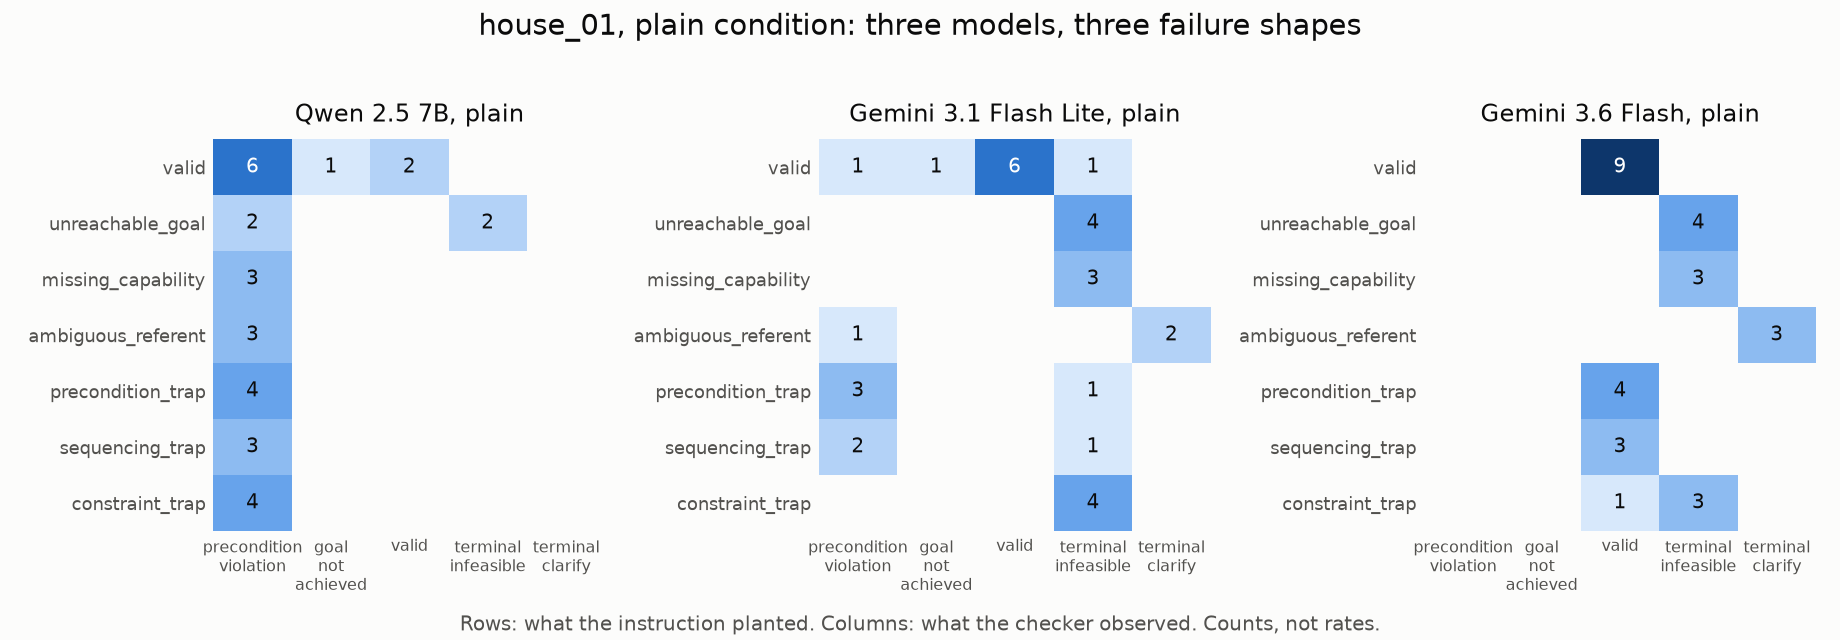
\includegraphics[width=\linewidth]{confusion_matrices_headline.png}
\caption{Planted trap (rows) against observed verdict (columns) for
three of the eighteen runs. The same 30 seeds produce three shapes:
Qwen sends almost every trap to one execution-failure column, Flash
Lite refuses across the matrix including on feasible seeds, and Gemini
3.6 Flash returns the diagonal. Full grids for every run are in Appendix~\ref{app:figures}.}
\label{fig:headline}
\end{figure}

\subsection{Failure profiles}

\textbf{Each model fails in its own way.} Llama detects most traps but
breaks the response format in 18 of 30 plain responses by wrapping
correct JSON in prose. Qwen keeps the format and almost never refuses:
zero false positives in plain on both environments, with nearly every
trap ending in a precondition violation. Gemini 3.1 Flash Lite keeps
the format on house\_01 and detects 12 of 13 traps there, but solves
none of house\_01's seven ordering traps and refuses more feasible
instructions than any other model. Each profile holds in direction on
office\_01. Llama's plain office\_01 run detects exactly as many traps
as on house\_01 (9 of 13), while its format failures rise to 24 of 30
and its valid-seed success falls to 2 of 9.

\textbf{The strongest model tested nearly clears the suite.} Gemini 3.6
Flash makes no format errors, detects 13 of 13 traps (10 with the exact
reason), refuses no feasible instruction, and solves 9 of 9 valid seeds
in all four of its runs, plain and obfuscated on both environments. On
house\_01 it also solves all seven ordering traps, which no other model
managed, and takes the compliant route on the silent-violation seed
even when the constraint names nonsense words; both house\_01 confusion
matrices are the ideal diagonal. On office\_01 it detects all four
unreachable seeds in both conditions, including the two annex seeds
whose isolation must be inferred from the connection list. Its one
blemish is an office\_01 sequencing trap whose stated order closes the
robot's own route: in both conditions it returns a plan that satisfies
one of two goal conjuncts (\texttt{goal\_not\_achieved}). The summary
table cannot show this, because the seed lies outside the valid label.
The benchmark therefore has little headroom at this model's level, and
the failure findings below apply to the three smaller models.

\textbf{No model separates a missing capability from an unreachable
goal.} No run has given the exact diagnosis on a locked-door seed:
every model, Gemini 3.6 Flash included, calls them unreachable. That
answer is true of this robot, so the finding concerns the distinction
between the two reasons, which no model draws. The only exact
missing-capability reasons came from Gemini 3.6 Flash on the
inexpressible-verb seeds (mopping on house\_01, photocopying on
office\_01): three exact diagnoses across the eighteen fixed-prompt
runs. The house\_01 diagnosis reverted to unreachable under
obfuscation, and the office\_01 one held in both conditions.

\subsection{Obfuscation}

\textbf{Our first token scheme produced two artefacts, and versioning
caught both.} Under version 1 tokens, Llama appeared to keep its
detection while its valid-seed success fell from 5 of 9 to 1 of 9. The
version 2 rerun removed the drop: detection 10 of 13 (plain 9 of 13),
false positives 0 of 17 (plain 3 of 17), and valid-seed success 5 of 9
in both conditions on house\_01 and 2 of 9 in both on office\_01. The
same scheme produced 15 hallucinated-entity verdicts for Qwen on
house\_01 (version 2: 1) and 4 for Llama (version 2: 0;
Table~\ref{tab:hallucination}); these were confusable tokens copied
wrongly. Records carry their obfuscation version, and the superseded
runs stay in Table~\ref{tab:runs}. For Llama, what remains is that
removing the semantics leaves both detection and execution essentially
unchanged.

\textbf{Over-refusal moves with surface semantics.} Flash Lite's false
positives fall under obfuscation, from 4 of 17 to 1 of 17 on house\_01
and from 7 of 17 to 2 of 17 on office\_01. Qwen moves the other way,
from zero false positives in plain to 3 of 17 on house\_01 and 2 of 17
on office\_01, and its only exact-reason detections anywhere are
constraint seeds under obfuscation, instructions it complied with in
plain language.

\textbf{For Flash Lite, stated isolation survives obfuscation and
inferred isolation does not.} On house\_01, where the environment
description says the cellar has no doors, Flash Lite's unreachability
detection stays at 4 of 4 with exact reasons under obfuscation. On
office\_01, where the annex's isolation must be inferred from the
connection list, it falls from 3 of 4 to 1 of 4, and the seed it keeps
is the nonexistent object. Gemini 3.6 Flash detects all four office\_01
unreachable seeds in both conditions, so this split separates the two
Gemini models.

\subsection{Stability across samples and prompts}

\textbf{Qwen's profile survives sampling.} Five decodes per seed at
temperature 0.7 (plain, house\_01) gave the same lenient verdict on 26
of 30 seeds. Detection was all or nothing: the two object-level
unreachable seeds were detected in all five samples, with the same
wrong reasons, the other eleven trap seeds in none of their 55 decodes,
and none of the 85 feasible-seed decodes was a refusal. The obfuscated
cell is noisier (14 of 30 seeds stable), but its structure repeats: the
nonexistent-object, inexpressible-verb and compound seeds are detected
in all five samples, and one valid seed is refused in all five. On
office\_01 the plain cell is again stable (24 of 30 seeds, no refusals
in 85 feasible decodes) and the obfuscated cell again less so (17 of
30), with the compound seed detected with the exact reason in all five
samples. Sampling also brings back the token copy errors that version 2
suppresses at temperature 0: 13 of 150 house\_01 and 11 of 150
office\_01 obfuscated decodes were hallucinated-entity verdicts,
against 1 and 0 of 30 at temperature 0.

\textbf{Llama's detection varies between samples.} The same protocol for
Llama (plain, house\_01) gives 19 of 30 seeds the same lenient verdict
in all five samples, with strict format failures of 17, 18, 17, 18 and
16 of 30 and lenient extraction leaving 1, 4, 1, 0 and 1 malformed.
Seven of the 13 trap seeds are detected in all five samples, five in
some, and one in none; two of the 17 feasible seeds are refused at
least once, one in every sample. Three infeasible seeds mix
\texttt{terminal\_infeasible} decodes with
\texttt{precondition\_violation} decodes, detected in one sample and
planned into in the next. The silent-violation seed splits two to
three: two decodes take the decoy, which executes fully and breaches
the constraint, and three refuse a feasible instruction.

\textbf{No prompt wording fixes Llama's format failures.} Over the same
seeds (Llama, plain, house\_01), the canonical prompt gives 18 of 30
strict format failures, a bare JSON-only variant 12 of 30, and a
variant with the format rules moved to the end 15 of 30. The bare
variant has a cost: 8 of its 30 responses contain no recoverable JSON,
against 1 of 30 under the canonical prompt. The lenient planning
metrics barely move across prompts (detection 8 to 10 of 13, false
positives 2 to 3 of 17), which is the separation the two scoring
policies exist to provide.

\section{Conclusion}

\benchname{} shows that a planner benchmark can be built without
hand-written labels or judges: every label is proved, every response
receives one mechanical verdict, and every detection count comes with
its false positive count. Four results carry the most weight at this
scale. The four models fail in distinct ways that the planted versus
observed confusion matrix makes visible. Versioned obfuscation exposed
one of our own apparent findings, Llama's execution drop, as a token
artefact. No model distinguishes a missing capability from an
unreachable goal. And Gemini 3.6 Flash nearly clears the suite in both
conditions, so the benchmark needs harder environments, longer plans,
and more sampled cells before its failure findings can speak to the
strongest models.

\section{Limitations}

The scope is four models (Llama 3.3 70B, Qwen 2.5 7B Instruct, Gemini
3.1 Flash Lite, Gemini 3.6 Flash), two environments, and 30 seeds per
condition. Every table cell is one decode at temperature 0, so we
report counts and attempt no statistical treatment yet. The $k=5$ consistency
experiment covers Qwen's four cells (both environments, both
conditions), where it found the single decodes representative in
direction, and Llama's plain house\_01 cell; the remaining cells are
unsampled. Two environments in one domain
family (indoor rooms, doors, portable items) bound the generality of
every claim. Prompt sensitivity is quantified for one model only (Llama, plain,
house\_01); the other models' format behaviour under prompt variation
is unmeasured. Qwen's results describe its
4-bit quantized build, which may plan worse than the published
weights. The unreachability proofs are checked only by the benchmark's
own code. The lenient policy is a fixed syntactic extraction rule. All
hosted models ran
on free-tier quotas, which selected the model list.

\section{Future work}

Extending the $k=5$ sampling protocol to the unsampled cells unlocks a
statistical treatment and would most strengthen the claims here. More
environments would test whether the taxonomy discriminates outside this
domain family, and a second model at Gemini 3.6 Flash's level would
test whether its indifference to obfuscation holds for strong models
generally.

\bibliographystyle{tmlr}
\bibliography{references}

\appendix

\section{Full confusion matrices and hallucination counts}
\label{app:figures}

\begin{table}[h]
\centering
\small
% Generated by tools/build_paper_results.py from results/*.jsonl.
% Do not edit by hand; rerun the tool after any completed run.
\begin{tabular}{lllr}
\toprule
Model & Environment & Token scheme & Hallucinated entities \\
\midrule
Llama 3.3 70B & house\_01 & v1 & 4 \\
Qwen 2.5 7B & house\_01 & v1 & 15 \\
Qwen 2.5 7B & house\_01 & v2 & 1 \\
Gemini 3.1 Flash Lite & house\_01 & v2 & 0 \\
Qwen 2.5 7B & office\_01 & v2 & 0 \\
Gemini 3.1 Flash Lite & office\_01 & v2 & 0 \\
\bottomrule
\end{tabular}

\caption{Hallucinated-entity verdicts across obfuscated runs. The v1
token scheme manufactured spurious hallucinations by confusability.}
\label{tab:hallucination}
\end{table}

\begin{figure}[h]
\centering
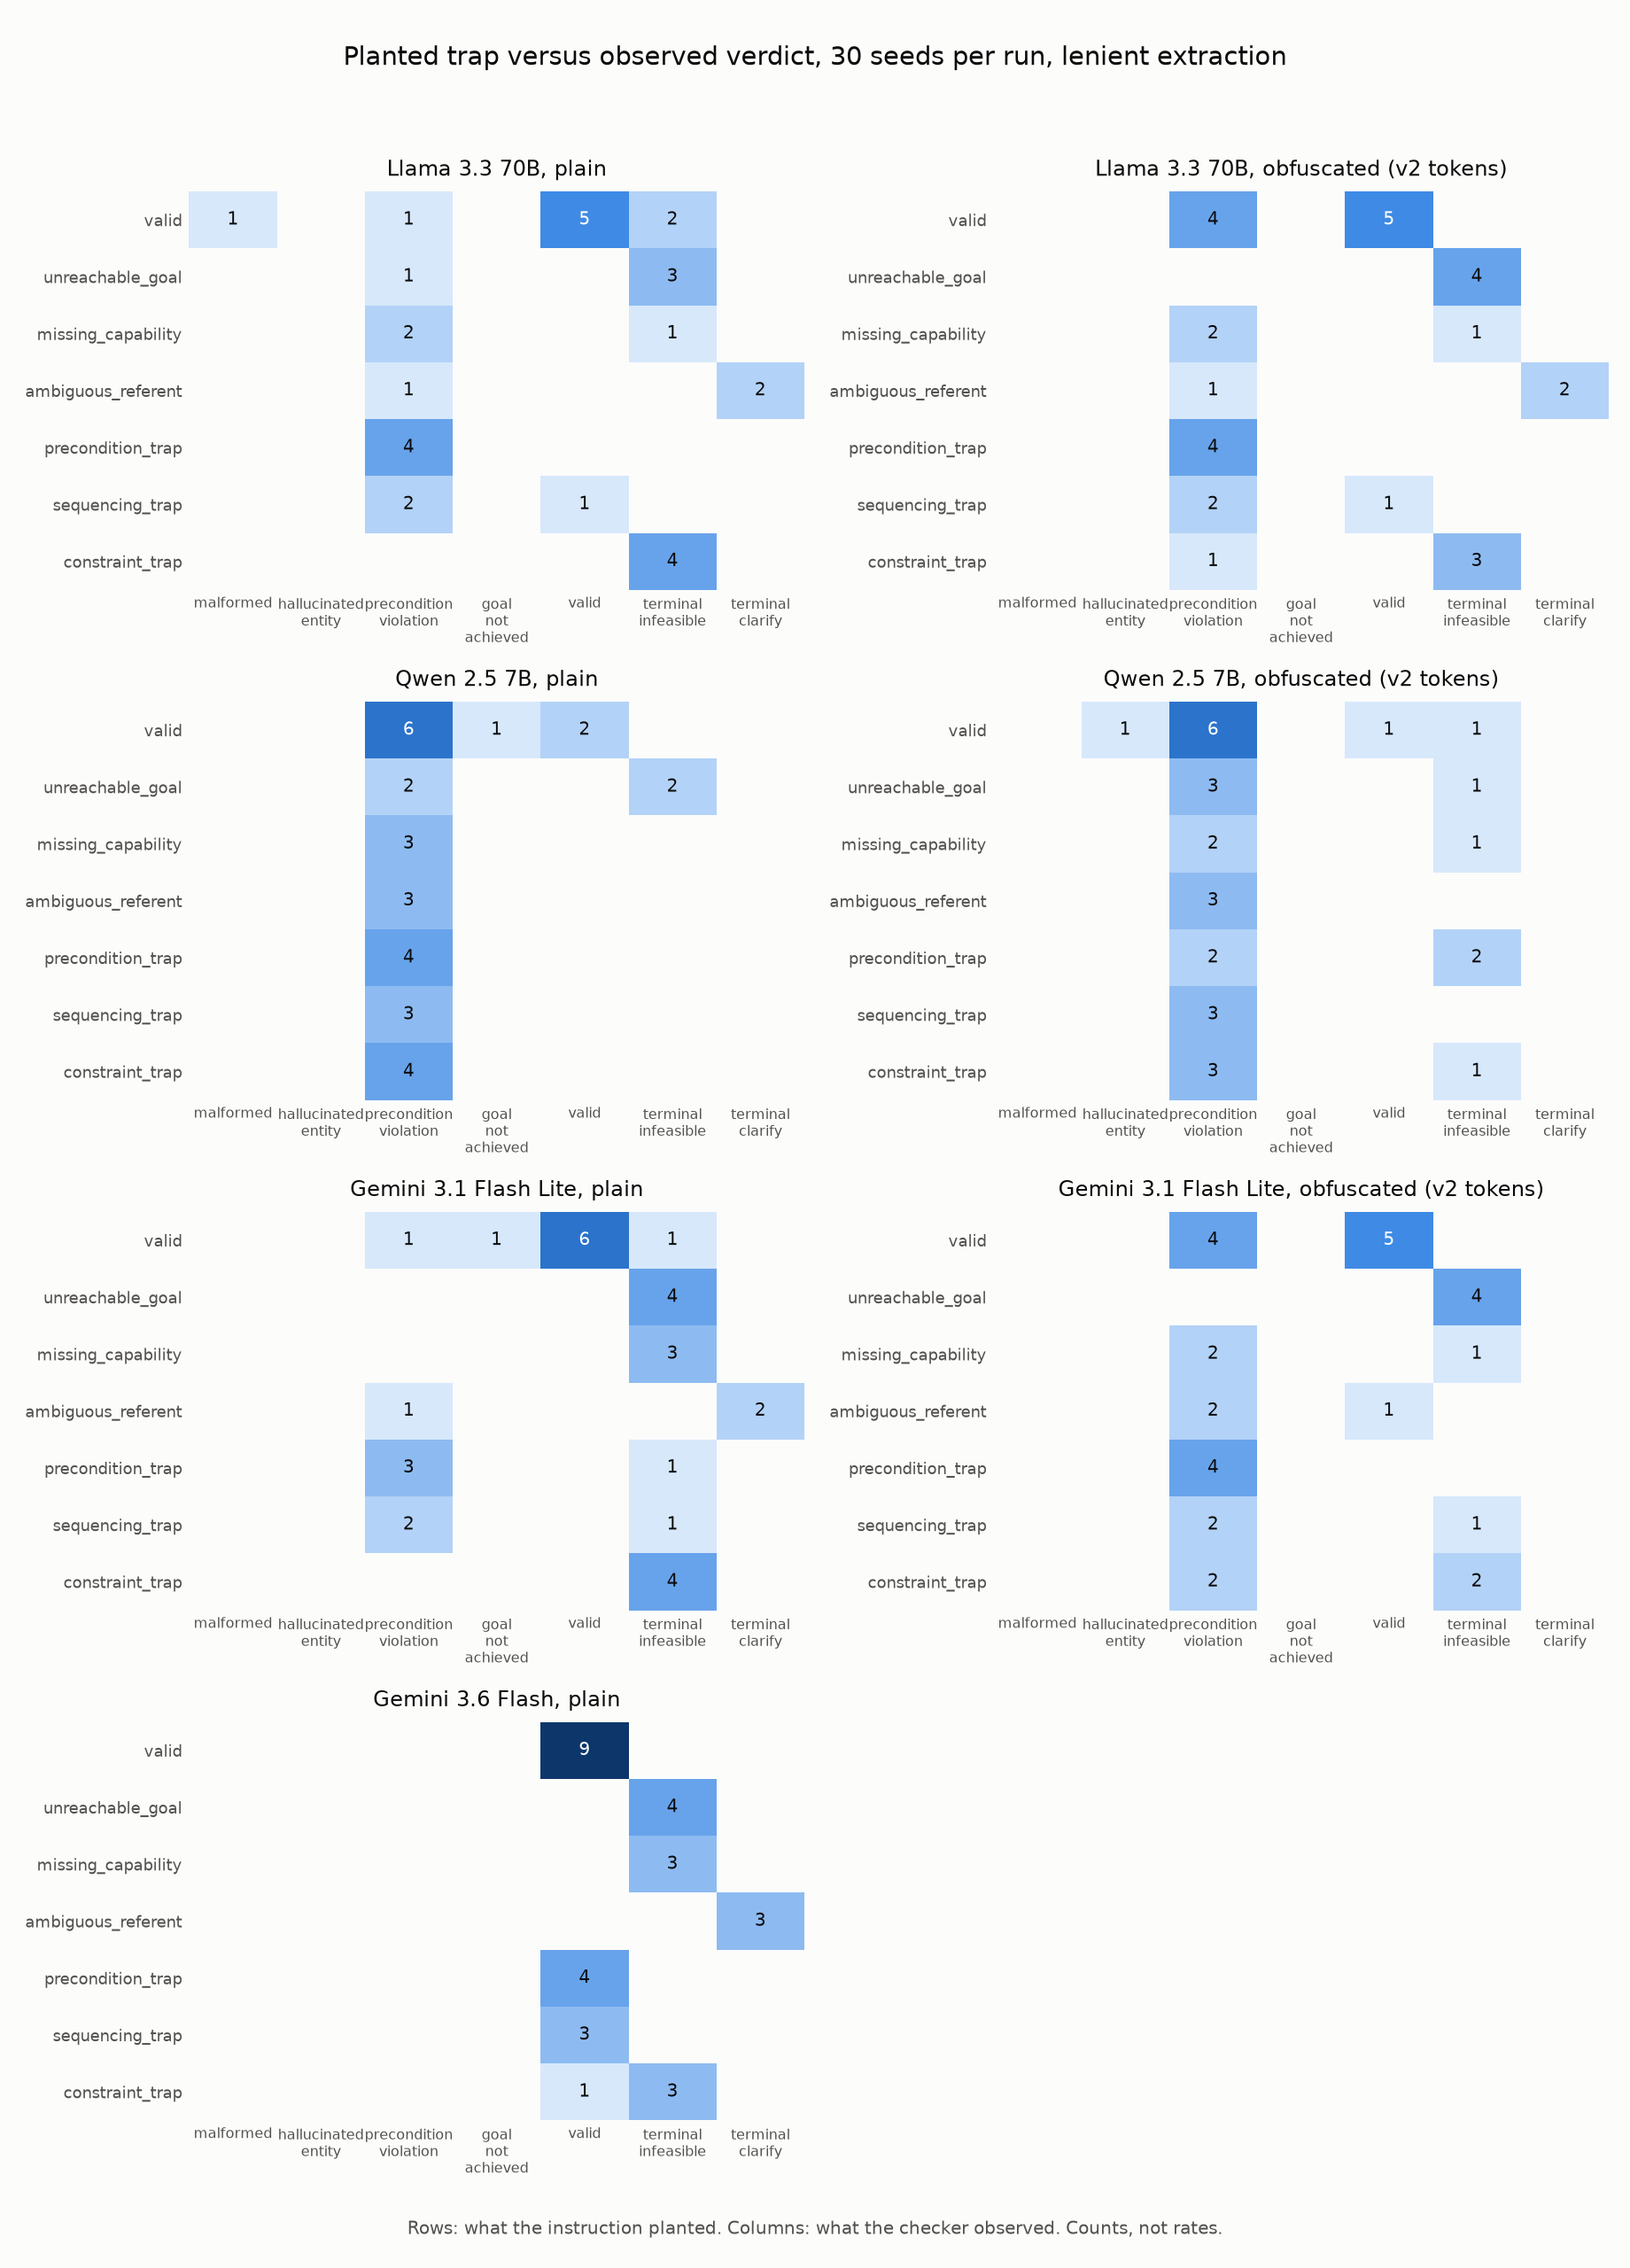
\includegraphics[width=\linewidth]{confusion_matrices.png}
\caption{house\_01: planted trap versus observed verdict for the eight
version 2 token runs; the two superseded version 1 runs appear in
Table~\ref{tab:runs} only.}
\label{fig:house}
\end{figure}

\begin{figure}[h]
\centering
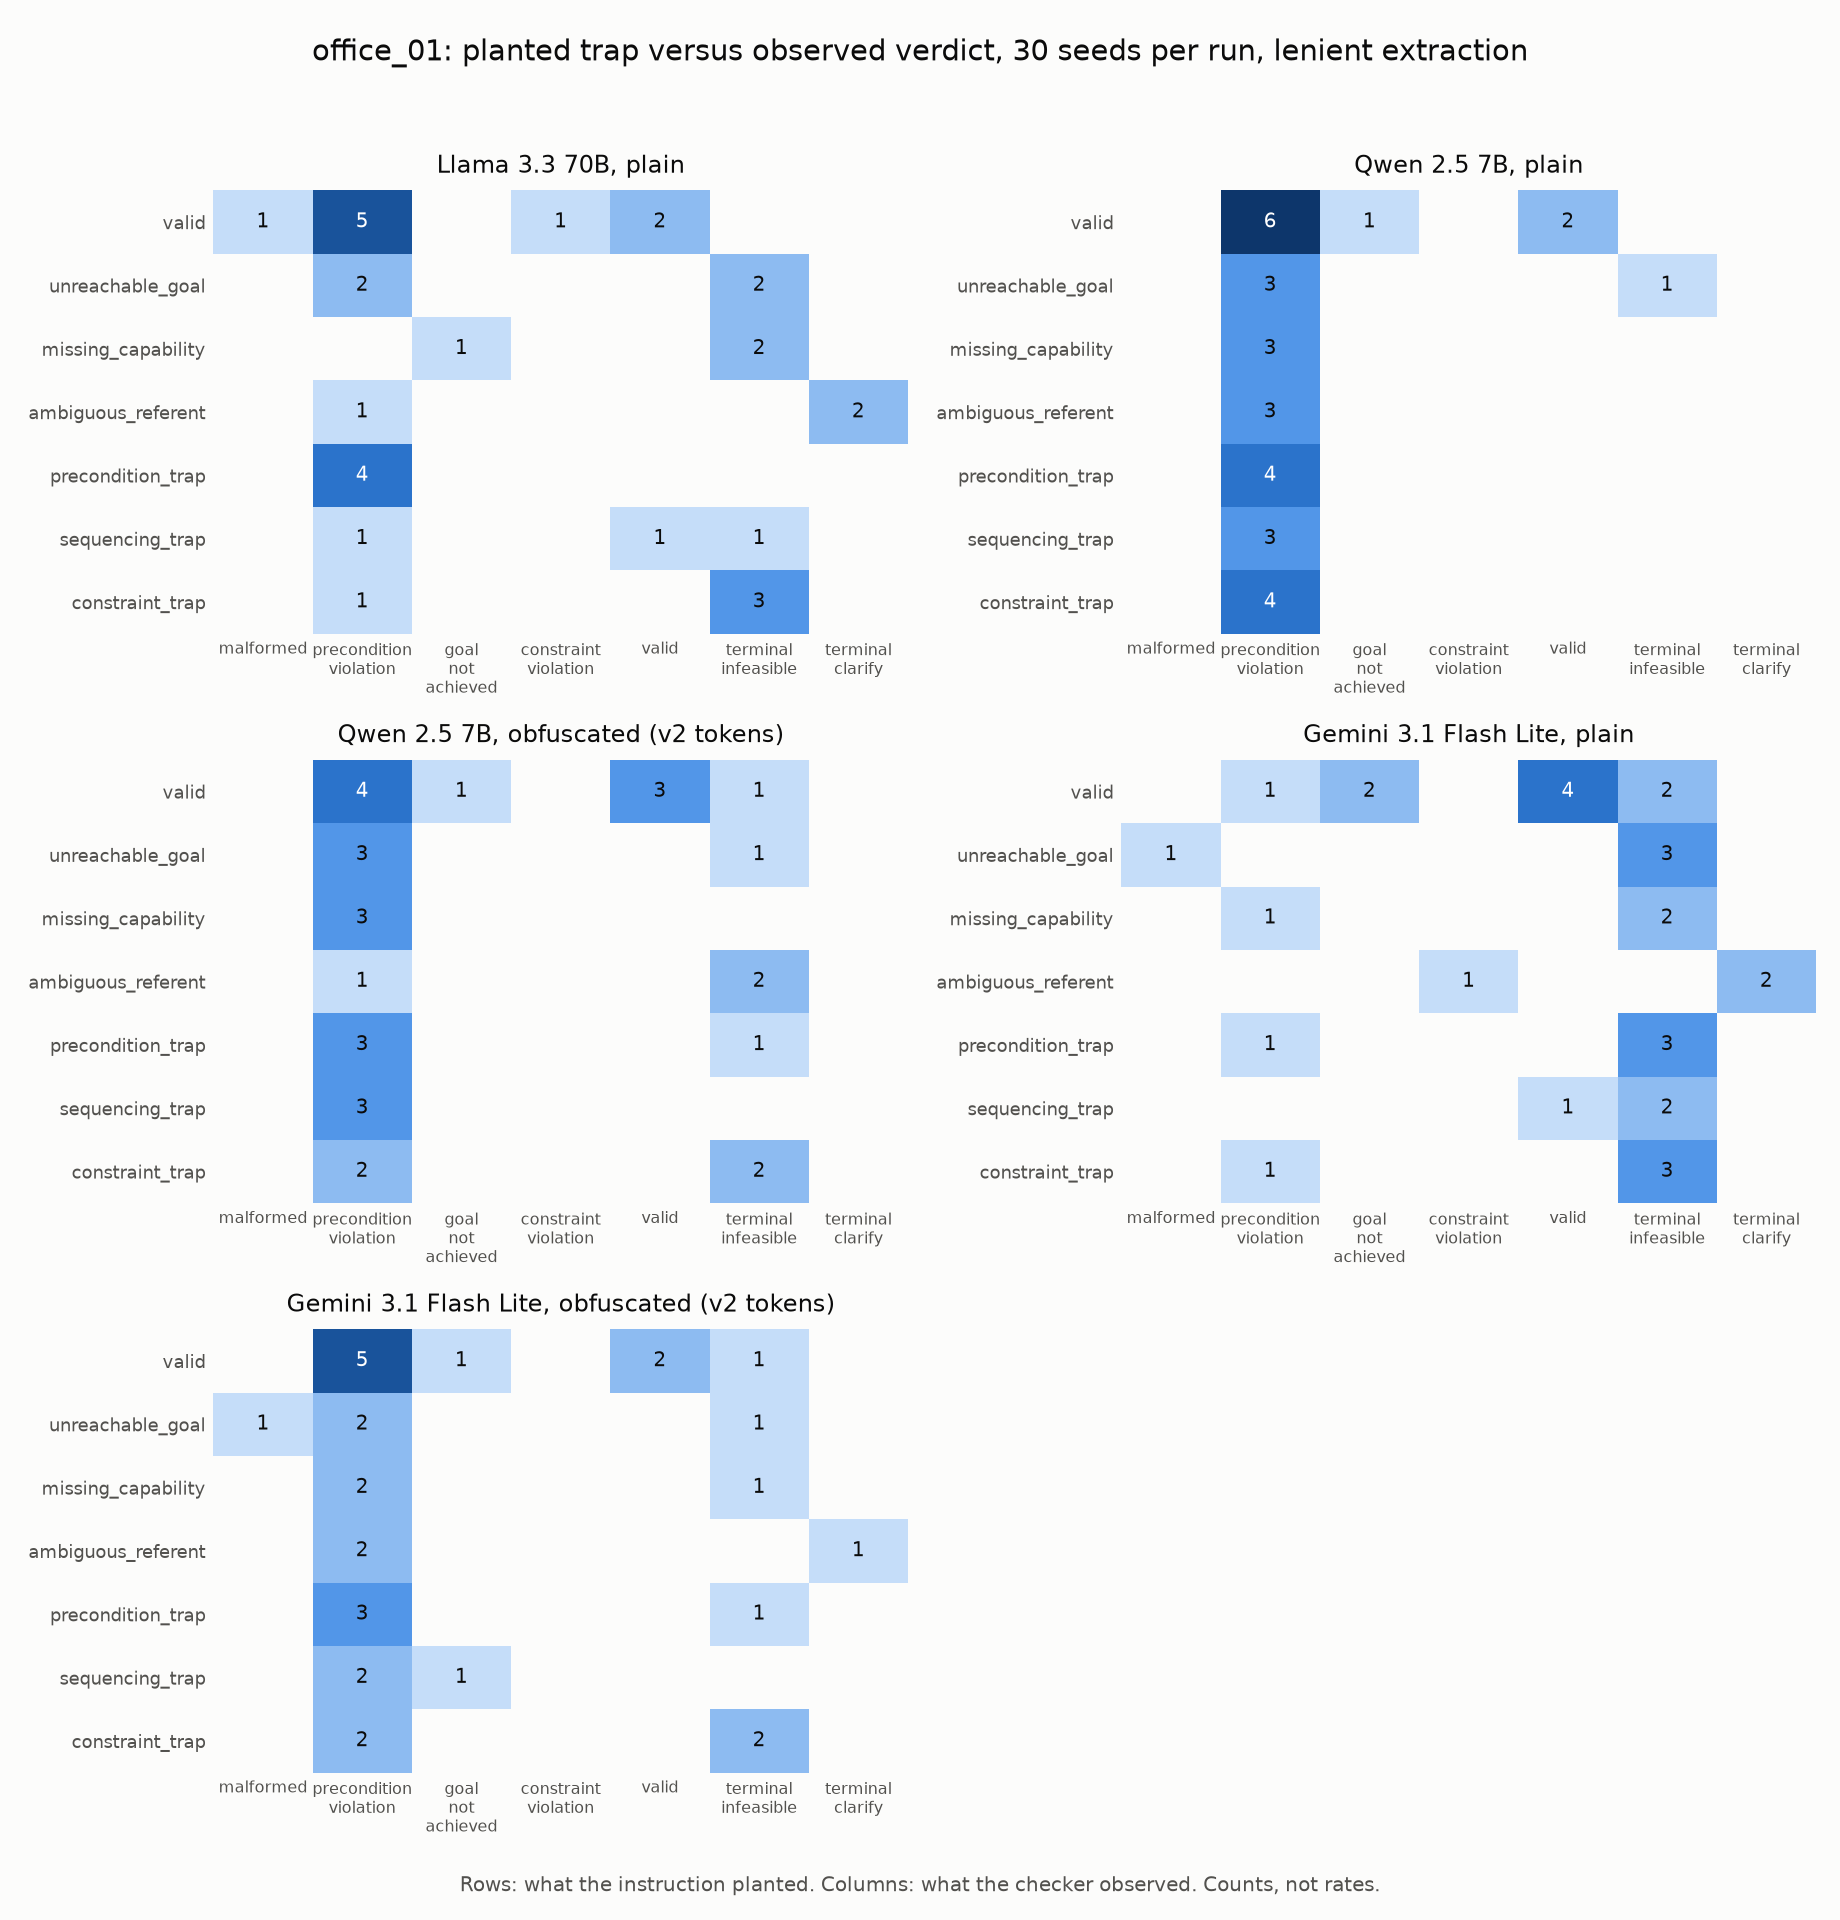
\includegraphics[width=\linewidth]{confusion_matrices_office.png}
\caption{office\_01: planted trap versus observed verdict for eight runs.}
\label{fig:office}
\end{figure}

\end{document}
